\begin{figure*}%[!hbtp]
	\centering
	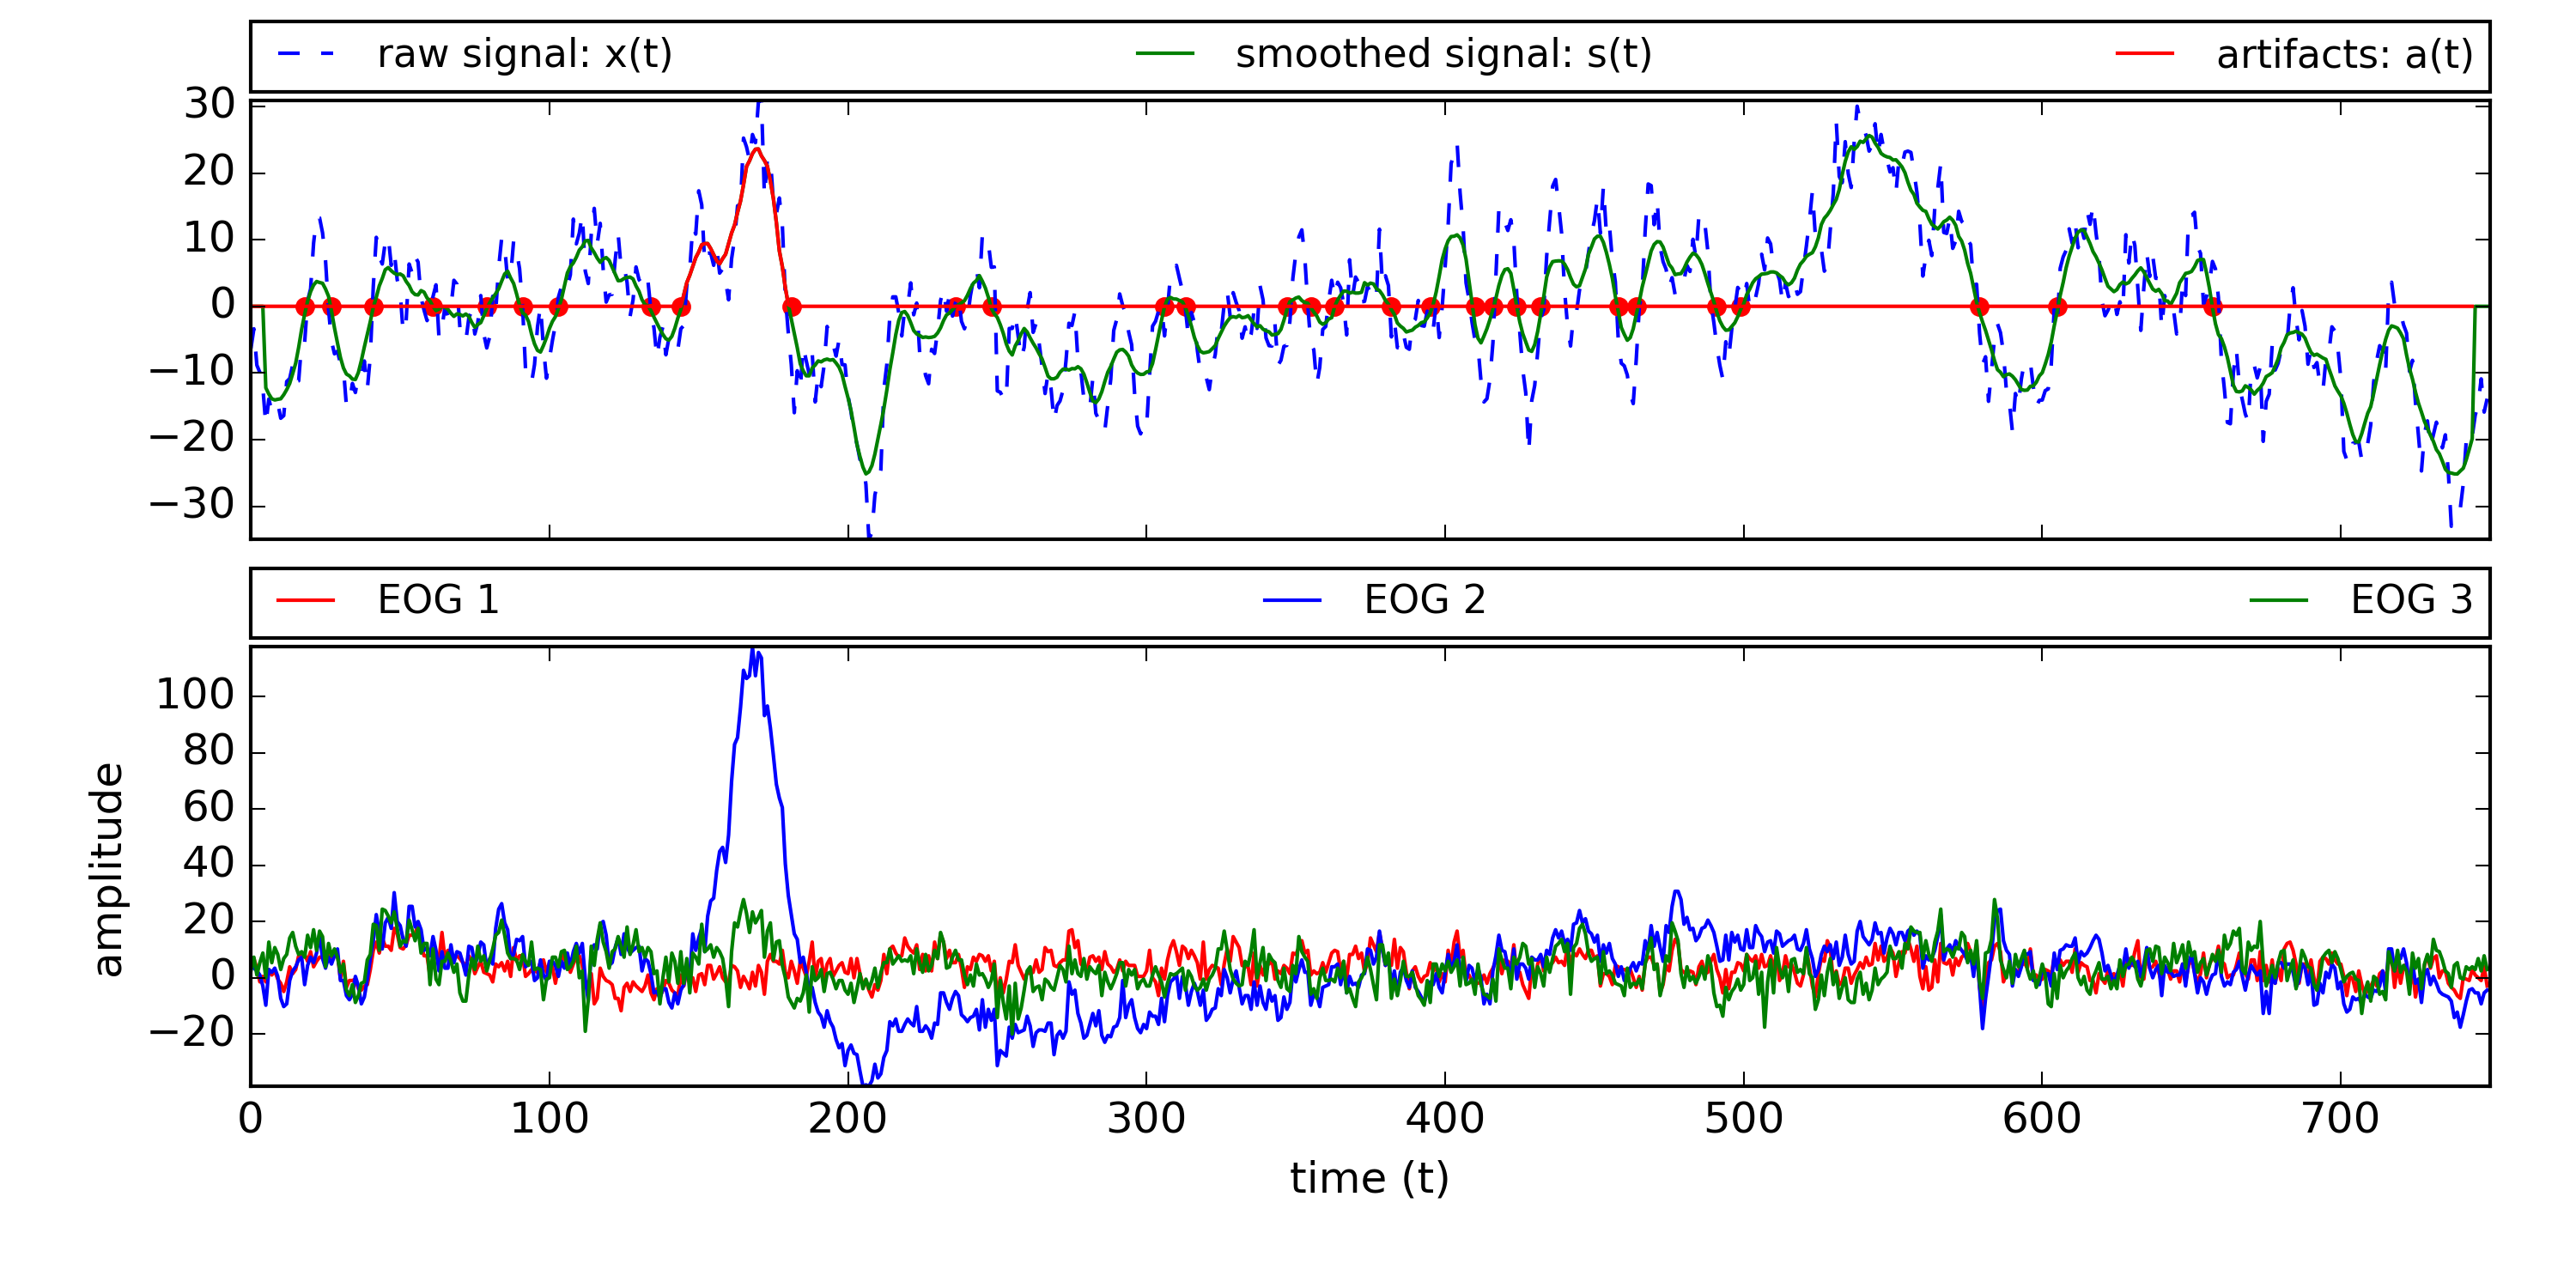
\includegraphics[width=1\textwidth]{figures/oacl-signals.png}
	\vspace{-2em}
	\label{fig:oacl-signals}
	\caption{Smoothed and artifact signal superimposed on the raw EEG signal for a single channel in part of a single trial.}
\end{figure*}
\section{Ocular Artifact Correction}\label{sec:oacl}
The OACL method consists of two parts. First, the raw EEG signals are processed to obtain the artifact signals, representing the parts of the signal that are artifacts. Then we find the \emph{filtering parameter} $\Theta$ for each the artifact signals, which determines the amount of each signal that are to be removed from the raw signal in order to obtain the corrected signal. 
Since the original OACL method \citep{li2015ocular} was devised for binary class datasets, we generalize the algorithm for multi-class datasets. 

Let $x = \{s_0, ...,s_n\}$ where $s_t \in \mathbb{R}_{\geq 0}$ denote the raw EEG data for some arbitrary channel. For simplicity, we can interpret $x$ as a function $x : \mathbb{N}_{\geq 0} \rightarrow \mathbb{R}_{\geq 0}$ where $x(t)$ denotes the amplitude of $x$ at time $t$. 
From $x(t)$ we perform all steps in artifact detection and removal.

%Let $t \in \mathbb{N}_{\geq 0}$ be the time of a EEG sample, then $x(t)$ denotes the amplitude measured at time $t$, that is, $x(t)$ denotes the raw EEG signal for some channel.

\subsection{Artifact Detection}
The goal of artifact detection is to find the artifact signal $a(t)$ from $x(t)$ that represents which parts of $x(t)$ that contains ocular artifactsare noise. Before finding the artifact signal $as(t)$, we first obtain a smoothed signal by applying a \emph{moving average filter} to $x(t)$, in order to smooth out short-term fluctuations from e.g. external interference. A moving average filter is a function $s: \mathbb{N} \rightarrow \mathbb{R}$ that given time t, computes the average of the $\frac{m}{2}$ samples on either side of the tth sample. 
\begin{equation}
\label{eq:movavg}
s(t) = \frac{1}{m}\sum_{t-\frac{m}{2}}^{t+\frac{m}{2}}x(t)
\end{equation}
where $m$ is the number of neighboring points used. The smoothed signal $s(t)$ shown together with the raw signal $x(t)$ are illustrated in \cref{fig:oacl-signals}.

From the smoothed signal $s(t)$ the OACL methodOACL finds the changes in amplitude between the samples, which could indicate eye movement. Therefore, we proceed by computing the relative heights between samples as the maximal difference in amplitude between a sample at time $t$ and its neighboring samples.
\begin{align*}
\Delta (t) = max(&|s(t)-s(t-1)|,\\
&|s(t+1) - s(t)|) \numberthis \label{eq:relheights}
\end{align*}
where we can consider $\Delta(t)$ as the describing the fluctuations in the signal.

Now, we want to have some measure of what an artifact signal looks like. \citet{li2015ocular} found by inspection that ocular artifacts generally occur with sudden changes in amplitude ($\Delta$) between $[30\mu V-50\mu V]$ and $[70\mu V-150\mu V]$. The problem with this approach is, that it does not generalize to data collected using different setups for the EEG measurement. For this reason, we automatically estimate the ranges by considering them parameters to be optimized through Bayesian Optimization, discussed in \cref{sec:bayesian-optimization}.
For now, assume that we have some arbitrary ranges
\begin{equation}\label{ranges}
R=[l, u] \quad  l,u \in \mathbb{N}_{\geq 0}
\end{equation}
then we can find the sample indexes $t$ where $\Delta (t)$  lies in the range $R$:
\begin{align*}
P = \{t \quad | \quad &\frac{m}{2} < t < n-\frac{m}{2}  \quad \textnormal{and} \\
& l < \Delta (t) < u\} \numberthis \label{eq:peaks}
\end{align*}
where $P$ is the indexes of the samples of the smoothed signal, where a change in amplitude lies within the range that characterizes an ocular artifact.

We now have the peaks of the ocular artifacts in $s(t)$, but we still need all of the artifact before we can correct it. The approach in the OACL method is to define the artifact to be from the closest zero point to the peak, before the peak, to the closest zero point after the peak. We can now find the artifact signal 
\begin{equation}
\label{eq:artifactsignal}
a(t) =
\begin{cases}
s(t)      & \quad \text{if } z_b \leq t < z_a\\
0  & \quad \text{otherwise}\\
\end{cases}
\end{equation}
where $z_b, z_a$ are the zero points after and before respectively. The concept of zero points of an artifact are illustrated in \cref{fig:oacl-signals}.

Zero points are found from the smoothed signal, by iterating through the list, finding crossovers from sample to sample. 
Let again $s(t)$ be the function for the smoothed signal defined in \cref{eq:movavg}. We now iterate through all values of $t$, where $t \in \{0,...,n\}$, finding all points $P$ where one of the following two conditions are true.
\begin{equation}
\label{eq:zero_points}
P =
\begin{cases}
s(t)      & \quad \text{if } s(t) \leq 0 \leq s(t + 1)\\
s(t + 1)  & \quad \text{if } s(t) \geq 0 \geq s(t + 1)\\
\end{cases}
\end{equation}
$P$ will then be a list of zero points $\{p_1,...p_m\}$, which are used as the indexes $z_a$ and $z_b$ in \cref{eq:artifactsignal}, to find artifact signals..

Recalling that we can use an arbitrary number of ranges in \cref{eq:ranges}, we obtain the set of artifact signals for a single channel of a single trial as:
\begin{equation}\label{eq:artifact-signals}
A(t)=  \begin{pmatrix}
a_1(t) \\
a_2(t) \\
\vdots  \\
a_n(t) 
\end{pmatrix}
\end{equation}
The idea behind this, is that different types of artifacts can be found by using different kinds of ranges. 
\subsection{Artifact Removal}
With the artifact signal $a(t)$ extracted from the raw EEG data the next task is to remove the artifacts characterized by $a(t)$ from the original signal $x(t)$. Since signals are closed under subtraction we can obtain the corrected signal by subtracting the artifact signal from the raw EEG signal:
\begin{equation}\label{eq:corrected-signal}
c(t) = x(t) - \theta A(t)
\end{equation}
where $\theta \in \mathbb{R}_{\geq 0}$ is the \emph{filtering parameter}. Intuitively, $\theta$ is a factor that determines the "amount" of the artifact signal to subtract from the raw signal. 

The original approach of OACL is to obtain the $\theta$ parameter by training a binary logistic regression classifier with a modified hypothesis function with the latent variable derived from the power of the raw signal. Instead of this approach, we consider $\theta$ parameters as hyperparameters to the ocular artifact detection, which means that we can find the values for $\theta$ by optimizing them through the Bayesian Optimization algorithm. In short, this means that find the corrected signals for one subject as
\begin{align}\label{eq:corrected-signal}
C(t)=  \begin{pmatrix}
c_1(t) \\
\vdots  \\
c_{k}(t) 
\end{pmatrix}
\end{align}
where $kY$ is the number of channels of classes. By \cref{eq:corrected-signal} this means that we optimize over $k \times n$ $\theta$ parameters in bayesian optimization, where $n$ is the number of artifact sigals in \cref{eq:artifact-signals}. As we expect to remove 0-100\% of the artifact signal from the raw signal, we constraint the domain of the $\theta$ parameter to be between 0 and 1.  

